\section{Testing}

\subsection{Introduction}

In this chapter, the system test cases performed are listed in first section.
In the last two sections, all the problems found while testing the system will be presented. In more details they will be divided in two groups: Major issues and Minor issues, where the Major issues are problems that can't be fixed in a small amount of time and may lead to a general rethinking of the whole architecture of the system, while Minor issues are simple bugs that can be fixed in a small amount of time.
Since the source code came with a sufficient amount of unit testing, the testing phase focused on black box testing: this technique while not being automated is one of the best for testing the general system behavior and stability.

\subsection{System testing}
The following test cases have been performed. If nothing is specified, the test case is to be assume positively performed.

\begin{itemize}
\item User and TPC signup.
\item User and TPC login.
\item User modifies its personal data (\textit{with one exception for taxcode}, see later).
\item TPC formulation of  individual requests.
\item User accept or refuse individual request.
\item TPC visualization of individual data: \textit{this task can sometimes fail causing the app to crash}.
\item TPC formulation of group requests.
\item TPC visualization of group data.
\item TPC deletion of individual and group request.
\end{itemize}


In the application, the location of the user or the coordinates of his data is never displayed, neither in the user view nor in the TPC view. This basically misses the goals G1 and G3 as stated in the RASD.

\subsection{Major Issues}
The main major issue that came out from the testing phase derived from an architectural decision: the thick client with a local database and server with another persistent database. The advantage of this architecture is that the client doesn't require a permanent connection but on the other hand this architectural design is very dangerous and needs a lot of care since the changes between the two database have to be synchronized in order to avoid inconsistencies between the two.
One very simple case is the following one: there are two App connected to the server and logged with the same account. One of the two changes the profile name: this change is registered by the server, but the App running on the phone where the profile was not changed doesn't update, creating inconsistency between its local DB and the server.
Another case that can prove this behavior is changing the profile name, closing the app and then reopening it. For this case an example is provided below.
Another major issue that was noted while analyzing the project is the model used in the server DB. In this model there are tables that do not map real entities and could be removed: for example the user daily activities table can be replaced by doing queries for minimum or maximum values of the heart rate and the other kind of data.


\begin{figure}
\centering
\begin{subfigure}{.5\textwidth}
  \centering
   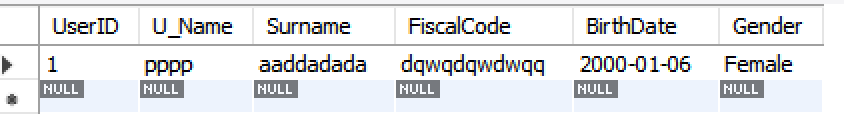
\includegraphics[scale=0.7]{resources/userdbnoupdate.png}
  \caption{Profile stored in the server}
  \label{fig:sub1}
\end{subfigure}%
\begin{subfigure}{.5\textwidth}
  \centering
   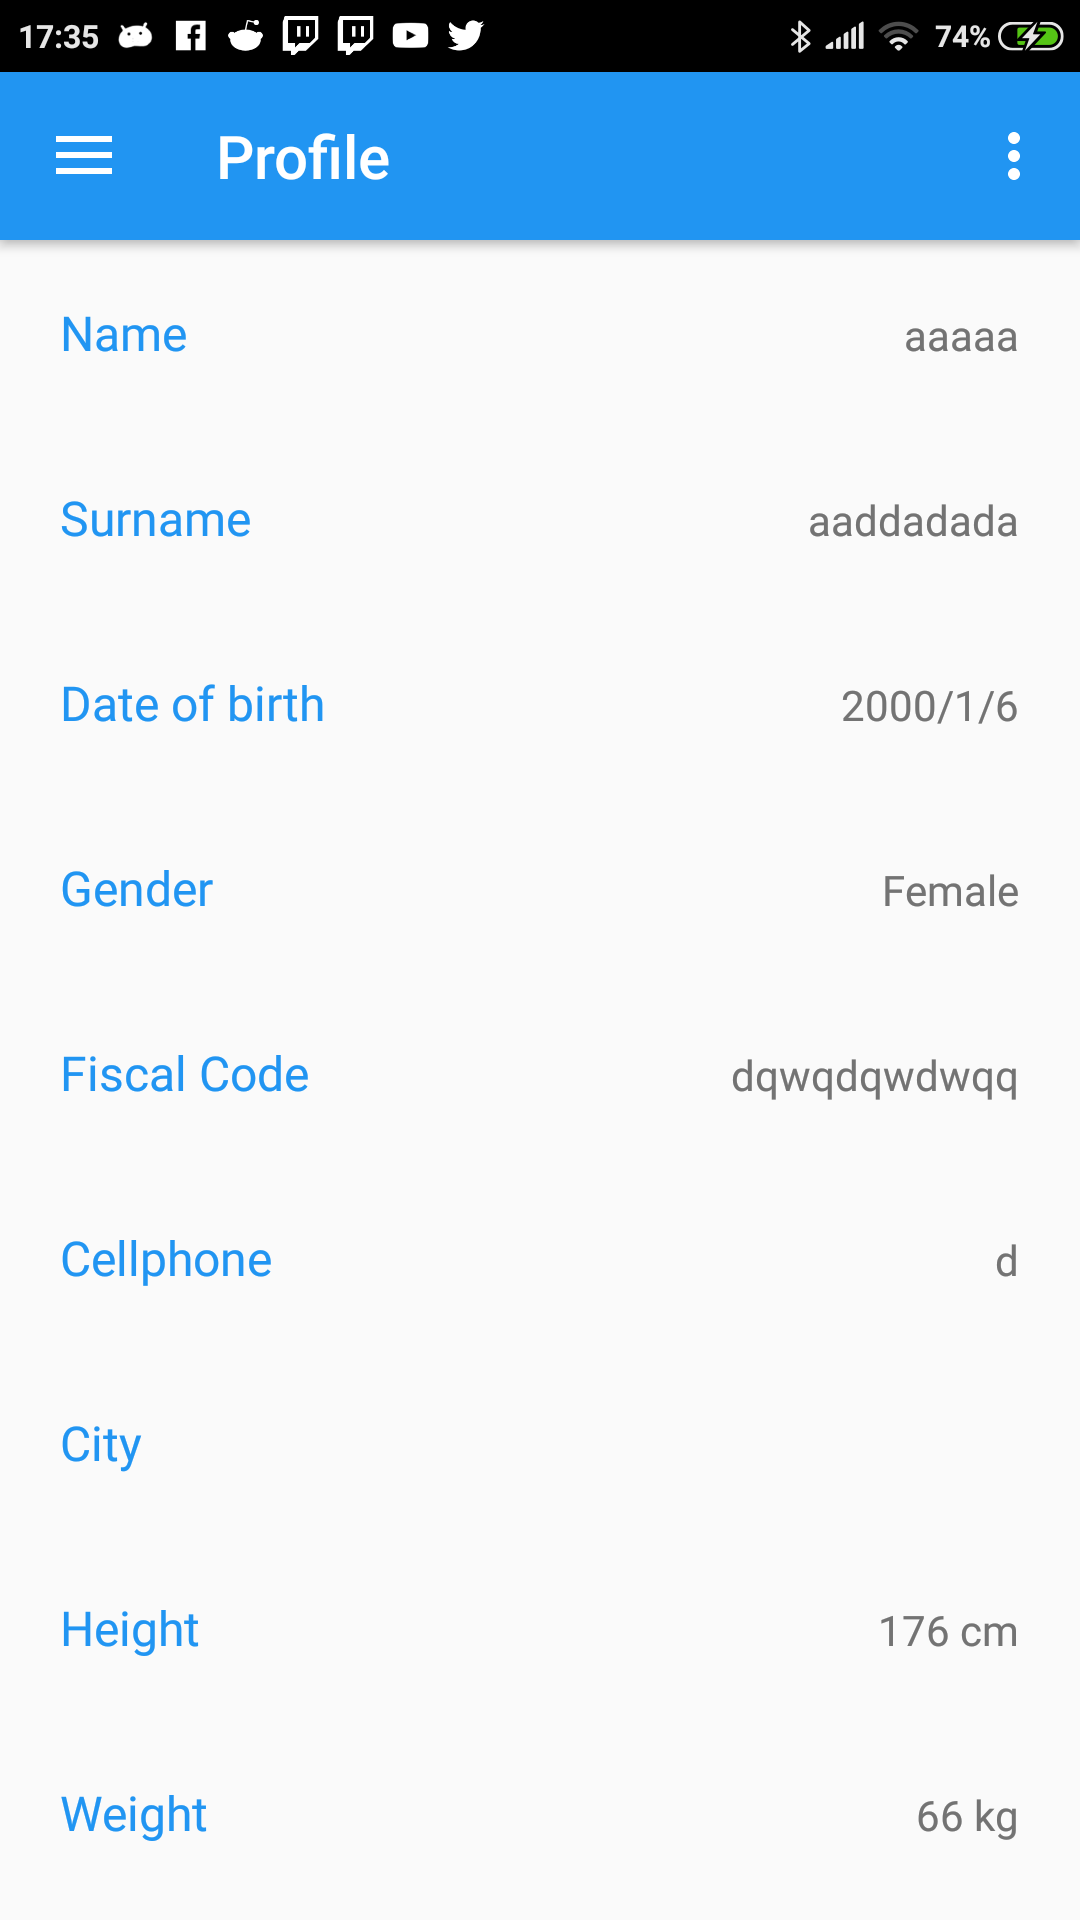
\includegraphics[scale=0.18]{resources/phoneprofile.png}
  \caption{Profile stored in the phone}
  \label{fig:sub2}
\end{subfigure}
\caption{Problem of inconsistency}
\label{fig:test}
\end{figure}

\subsection{Minor issues}
Here is a list of bugs that were noticed while testing the app, with the corresponding screenshots:
\begin{itemize}
\item[] In the login page, the notification for unsuccessful login doesn't have text or displays raw data coming from an html document.
\item[] In the profile page of the individual's App section no check is made on the user input, meaning that an user could set a random series of number and characters for its name, surname, cellphone and so on. This bug was presented because in the Signup Form instead there was a rigid check on the TC.
\item[] In the wearable page of the individual's App, editing the wearable name caused a crash of the app. The fix for this issue is presented in picture
\item[] The selection of countries for third parties and cities for individuals doesn't work
\item[] If a user tries to change its taxcode with a taxcode already present in the database, the application  crashes.
\item[] Sometimes, when trying to visualize the data about an individual who has accepted the request, the application crashes. This happens with some specific individuals, apparently without any reason. For example, we observed this issue with the individual in Figure \ref{fig:indiv_crash}.
\end{itemize}


\begin{figure}
\centering
\begin{subfigure}{.5\textwidth}
  \centering
   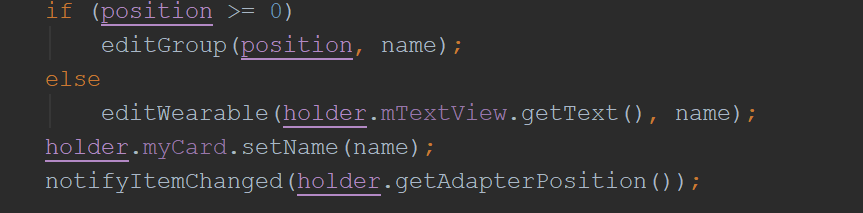
\includegraphics[scale=0.6]{resources/bugwearablwe.png}
   \caption{Part of the code that caused the crash while editing the wearable name}
  \label{fig:sub1}
\end{subfigure}%
\begin{subfigure}{.5\textwidth}
  \centering
   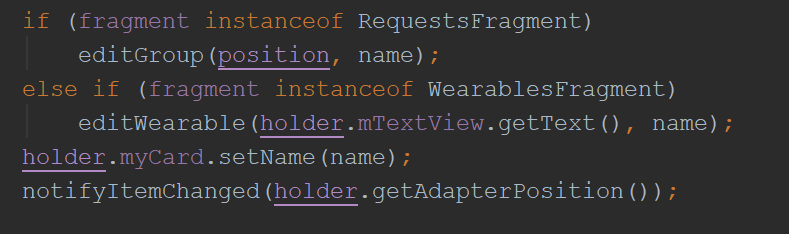
\includegraphics[scale=0.6]{resources/bugfixed.png}
   \caption{The fix implemented to make it work}
  \label{fig:sub2}
\end{subfigure}
\caption{Wearable edit name bug}
\label{fig:test}
\end{figure}

\begin{center}
   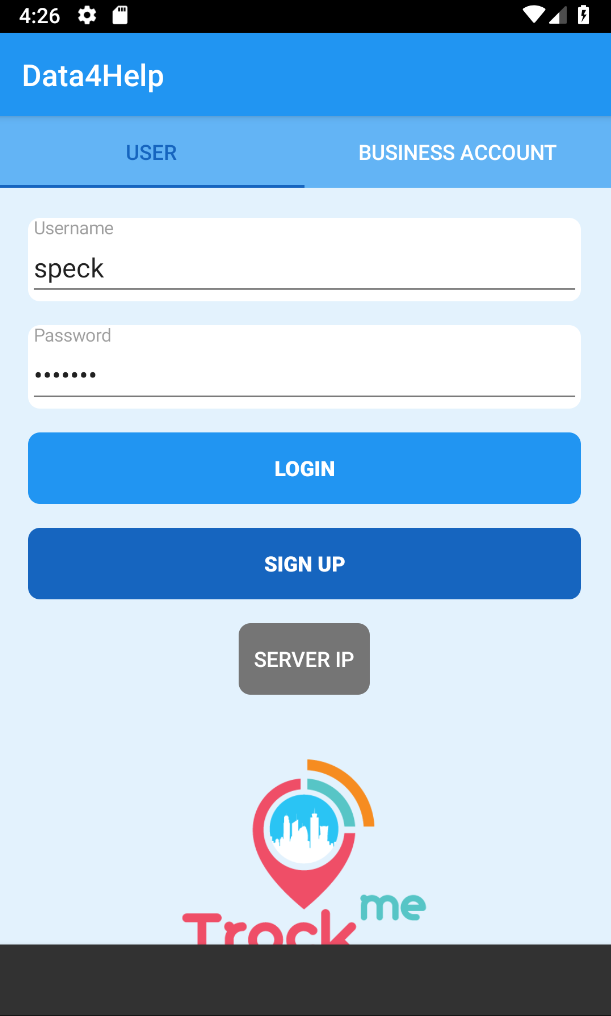
\includegraphics[scale=0.7]{resources/greybar.png}
   \captionof{figure}{Grey notification bar in the login page}
\end{center}

\begin{center}
   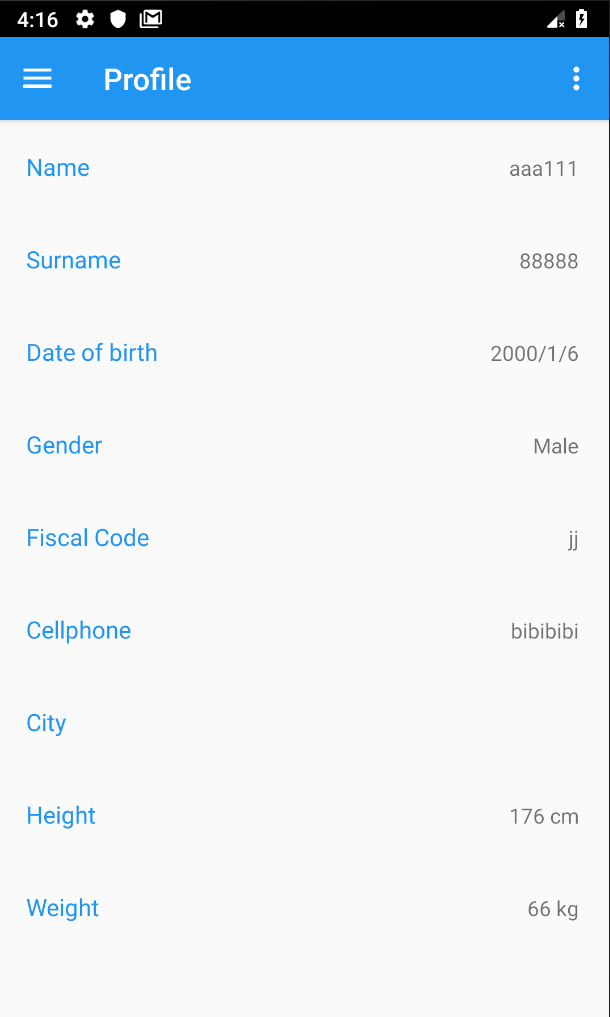
\includegraphics[scale=0.7]{resources/profilebug.png}
   \captionof{figure}{Example of profile input not checked}
\end{center}

\begin{figure}
\centering
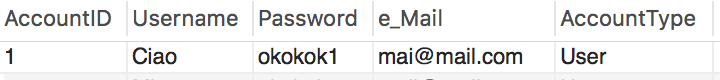
\includegraphics[scale=0.8]{resources/individual_crash}
\caption{Individual who causes the crash}\label{fig:indiv_crash}
\end{figure}
